\index{Romberg integration}
\index{Monte Carlo integration}
\chapter{Numerical Integration II --- Romberg \& Monte Carlo}
\newthought{Smarter Extrapolation and Escaping the Curse of Dimensionality}


% ==============================================================================================
% INTRODUCTION BLOCK

\section{The Why}
\index{Richardson extrapolation!motivation}

\newthought{In the previous chapter,} we learned that the trapezoid rule has error $O(h^2)$.
To halve the error, we need to double the number of points---quadrupling the work.
Can we do better?

\newthought{Richardson extrapolation} gives us a remarkable answer: by cleverly combining results from different step sizes, we can \emph{cancel error terms} and achieve higher accuracy \emph{without} evaluating $f$ at new points.

\newthought{But there's a bigger problem.} In $d$ dimensions, quadrature needs $N^d$ points.

\marginnote{\newthought{The curse of dimensionality:}
\begin{itemize}
    \item $d = 2$: $N^2 = 100$ points
    \item $d = 10$: $N^{10} = 10^{10}$ points
    \item $d = 100$: $N^{100} = 10^{100}$ points
\end{itemize}
Even $N = 10$ becomes impossible for high $d$. This is why high-dimensional problems require fundamentally different approaches.}

For $d = 100$ (common in ML), deterministic quadrature is hopeless.

\newthought{Monte Carlo integration} provides the escape: its error is $O(1/\sqrt{N})$ \emph{regardless of dimension}. This is why stochastic methods dominate high-dimensional problems.

\index{stochastic methods}
\newthought{In machine learning and artificial intelligence:}
\begin{itemize}
    \item \textbf{SGD is Monte Carlo:} $\nabla_\theta \mathbb{E}[L] = \mathbb{E}[\nabla_\theta L] \approx \frac{1}{|B|}\sum_{i \in B} \nabla_\theta \ell_i$
    \item \textbf{MC Dropout:} Uncertainty quantification via random dropout at test time
    \item \textbf{Variational inference:} ELBO estimated via MC samples
    \item \textbf{Policy gradients:} Reward expectations via trajectory sampling
    \item \textbf{Diffusion models:} Score function estimation uses MC
\end{itemize}

\newthought{Key insight:} Understanding Monte Carlo means understanding why SGD works and how to make it work better.



\newpage
\subsection{Hands On Experience}
\index{Richardson extrapolation!example}

\newthought{Richardson extrapolation magic:} We have trapezoid estimates with $n = 1$ and $n = 2$ intervals for $\int_0^1 e^x dx$:
\begin{align*}
    T_1 &= \frac{1}{2}[e^0 + e^1] = \frac{1 + e}{2} \approx 1.8591 \\
    T_2 &= \frac{0.5}{2}[e^0 + 2e^{0.5} + e^1] \approx 1.7539
\end{align*}

True value: $e - 1 \approx 1.7183$.

\vspace{1em}
\newthought{The extrapolation trick:} Since trapezoid error is $O(h^2)$, we can combine:
\begin{align*}
    T^* &= \frac{4 \cdot T_2 - T_1}{4 - 1} \\
    &= \frac{4(1.7539) - 1.8591}{3} \\
    &= \frac{7.0156 - 1.8591}{3} \\
    &= 1.7188
\end{align*}

\marginnote{\newthought{We jumped from} $O(h^2)$ to $O(h^4)$ accuracy using only the function values we already computed! No new evaluations needed.}

\newthought{Error comparison:}
\begin{table*}[ht]
\centering
\begin{tabular}{p{0.30\textwidth}p{0.20\textwidth}p{0.28\textwidth}}
\toprule
\textbf{Estimate} & \textbf{Value} & \textbf{Error} \\
\midrule
$T_1$ (1 interval) & 1.8591 & 0.141 (8.2\%) \\
$T_2$ (2 intervals) & 1.7539 & 0.036 (2.1\%) \\
$T^*$ (extrapolated) & 1.7188 & 0.0005 (0.03\%) \\
\bottomrule
\end{tabular}
\vspace{2em}
\caption{Richardson extrapolation dramatically improves accuracy without new function evaluations.}
\label{tab:richardson_comparison}
\end{table*}

The extrapolated value is 70$\times$ more accurate than $T_2$!


\vspace{2em}
\newthought{The Learning Objectives} of this chapter aim at providing you with the abilities to:
\begin{itemize}
    \item Derive and apply Richardson extrapolation to improve quadrature accuracy
    \item Construct and use the Romberg integration tableau
    \item Understand why the curse of dimensionality defeats deterministic methods
    \item Derive and apply Monte Carlo integration
    \item Use variance reduction techniques
    \item Connect MC methods to SGD and other ML techniques
\end{itemize}




% ==============================================================================================
% MAIN THEORY BLOCK

\newpage
\section{Richardson Extrapolation}
\index{Richardson extrapolation}

\newthought{The key observation:} For smooth functions, the trapezoid error can be written as a power series in $h^2$:
\begin{equation}
    T(h) = I + c_1 h^2 + c_2 h^4 + c_3 h^6 + \cdots
\end{equation}

where $I$ is the true integral and $c_i$ are constants that depend on $f$ but \emph{not} on $h$.

\marginnote{\newthought{Why only even powers?} The Euler-Maclaurin formula shows that trapezoid error involves only even powers of $h$ for periodic functions or functions with matching derivatives at endpoints.}

\newthought{With two step sizes} $h$ and $h/2$:
\begin{align}
    T(h) &= I + c_1 h^2 + c_2 h^4 + O(h^6) \\
    T(h/2) &= I + c_1 (h/2)^2 + c_2 (h/2)^4 + O(h^6) \\
    &= I + \frac{c_1 h^2}{4} + \frac{c_2 h^4}{16} + O(h^6)
\end{align}

\newthought{Eliminate the $h^2$ term:} Multiply the second equation by 4 and subtract:
\begin{align}
    4T(h/2) - T(h) &= 4I + c_1 h^2 + \frac{c_2 h^4}{4} - I - c_1 h^2 - c_2 h^4 + O(h^6) \\
    &= 3I - \frac{3c_2 h^4}{4} + O(h^6)
\end{align}

Solving for $I$:
\begin{equation}
    \boxed{T^*(h) = \frac{4 T(h/2) - T(h)}{4 - 1} = I + O(h^4)}
\end{equation}

\marginnote{\newthought{We jumped from} $O(h^2)$ to $O(h^4)$ without any new function evaluations! This is the power of extrapolation.}

\newthought{This is exactly Simpson's rule!} The weights $\frac{4}{3}$ and $-\frac{1}{3}$ that combine trapezoid estimates are the same as Simpson's rule weights. Richardson extrapolation reveals the deep connection.

\newthought{General Richardson extrapolation:} If a method has error $O(h^p)$:
\begin{equation}
    T^*(h) = \frac{2^p T(h/2) - T(h)}{2^p - 1} = I + O(h^{p+q})
\end{equation}

where $q$ depends on the error structure.




\newpage
\section{Romberg Integration}
\index{Romberg integration}

\newthought{Romberg's idea:} Apply Richardson extrapolation \emph{repeatedly} to build a tableau of increasingly accurate estimates.

\newthought{The Romberg tableau:}

\begin{center}
\begin{tabular}{c|cccc}
Step size & $O(h^2)$ & $O(h^4)$ & $O(h^6)$ & $O(h^8)$ \\
\hline
$h$ & $T_{0,0}$ & & & \\
$h/2$ & $T_{1,0}$ & $T_{1,1}$ & & \\
$h/4$ & $T_{2,0}$ & $T_{2,1}$ & $T_{2,2}$ & \\
$h/8$ & $T_{3,0}$ & $T_{3,1}$ & $T_{3,2}$ & $T_{3,3}$ \\
\end{tabular}
\end{center}

\marginnote{\newthought{Reading the tableau:}
\begin{itemize}
    \item Column 0: trapezoid rule
    \item Column 1: Simpson's rule accuracy
    \item Column 2: Boole's rule accuracy
    \item Diagonal: best estimates
\end{itemize}}

\newthought{Recurrence relation:}
\begin{equation}
    \boxed{T_{i,j} = \frac{4^j T_{i,j-1} - T_{i-1,j-1}}{4^j - 1}}
\end{equation}

For $j = 1$: $T_{i,1} = \frac{4 T_{i,0} - T_{i-1,0}}{3}$ (eliminates $h^2$ term)

For $j = 2$: $T_{i,2} = \frac{16 T_{i,1} - T_{i-1,1}}{15}$ (eliminates $h^4$ term)


\subsection{Detailed Example}
\index{Romberg integration!example}

\newthought{Compute} $\int_0^1 e^x dx = e - 1 \approx 1.718281828$ using Romberg.

\textbf{Column 0 (trapezoid):}
\begin{align*}
    T_{0,0} &= \frac{1}{2}[f(0) + f(1)] = \frac{1 + e}{2} = 1.859141 \\
    T_{1,0} &= \frac{1}{4}[f(0) + 2f(0.5) + f(1)] = \frac{1 + 2e^{0.5} + e}{4} = 1.753931 \\
    T_{2,0} &= \frac{1}{8}[f(0) + 2f(0.25) + 2f(0.5) + 2f(0.75) + f(1)] = 1.727222
\end{align*}

\textbf{Column 1 (extrapolated):}
\begin{align*}
    T_{1,1} &= \frac{4 \cdot 1.753931 - 1.859141}{3} = 1.718861 \\
    T_{2,1} &= \frac{4 \cdot 1.727222 - 1.753931}{3} = 1.718319
\end{align*}

\textbf{Column 2 (extrapolated again):}
\begin{align*}
    T_{2,2} &= \frac{16 \cdot 1.718319 - 1.718861}{15} = 1.718283
\end{align*}

\begin{center}
\begin{tabular}{c|ccc}
$n$ & $T_{i,0}$ & $T_{i,1}$ & $T_{i,2}$ \\
\hline
1 & 1.859141 & & \\
2 & 1.753931 & 1.718861 & \\
4 & 1.727222 & 1.718319 & 1.718283 \\
\end{tabular}
\end{center}

With only 5 function evaluations, $T_{2,2}$ matches the exact answer to 5 decimal places!

\newthought{Convergence:} For smooth functions, the diagonal elements converge extremely fast---often reaching machine precision with just a few rows.




\newpage
\section{The Curse of Dimensionality}
\index{curse of dimensionality}

\newthought{For $d$-dimensional integrals:}
\begin{equation}
    I = \int_{\Omega} f(\mathbf{x}) \, d\mathbf{x}, \quad \Omega \subset \mathbb{R}^d
\end{equation}

\newthought{Tensor product quadrature:} Apply 1D rule in each dimension independently.

With $N$ points per dimension, total points needed: $N^d$.

\begin{figure}[h]
    \centering
    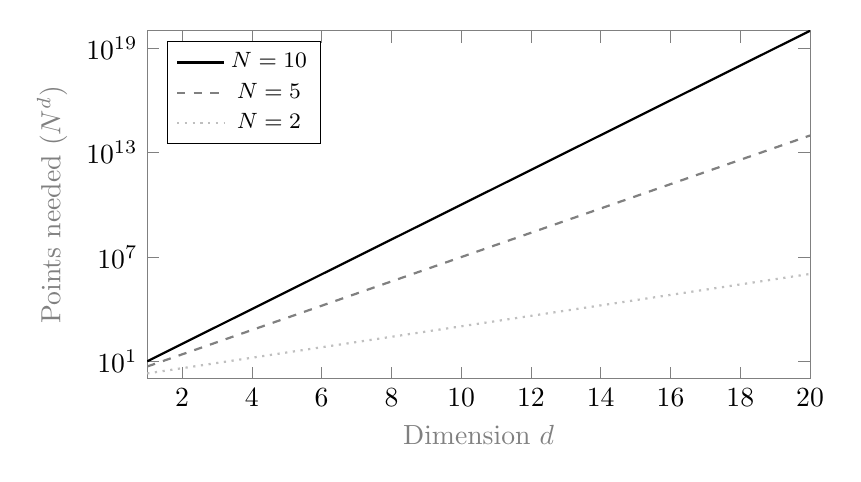
\begin{tikzpicture}
        \begin{axis}[
            width=10cm,
            height=6cm,
            xlabel={Dimension $d$},
            ylabel={Points needed ($N^d$)},
            ymode=log,
            xmin=1, xmax=20,
            ymin=1, ymax=1e20,
            tick style={gray},
            label style={gray},
            axis line style={gray},
            legend pos=north west,
            legend style={font=\footnotesize},
        ]
        \addplot[black, thick, domain=1:20, samples=20] {10^x};
        \addlegendentry{$N = 10$}
        \addplot[gray, thick, dashed, domain=1:20, samples=20] {5^x};
        \addlegendentry{$N = 5$}
        \addplot[gray!50, thick, dotted, domain=1:20, samples=20] {2^x};
        \addlegendentry{$N = 2$}
        \end{axis}
    \end{tikzpicture}
    \caption{Points needed for tensor product quadrature grow exponentially with dimension, regardless of $N$.}
    \label{fig:curse_dim}
\end{figure}

\marginnote{\newthought{Machine learning context:} A neural network with $d = 10^6$ parameters would need $(N)^{10^6}$ grid points---even $N = 2$ gives $2^{10^6}$, a number with 300,000 digits.}

\newthought{Concrete numbers:}
\begin{table*}[ht]
\centering
\begin{tabular}{p{0.20\textwidth}p{0.28\textwidth}p{0.20\textwidth}}
\toprule
\textbf{Dimension $d$} & \textbf{Points ($N=10$)} & \textbf{Status} \\
\midrule
2 & 100 & Easy \\
5 & 100,000 & Doable \\
10 & $10^{10}$ & Hard \\
20 & $10^{20}$ & Impossible \\
100 & $10^{100}$ & Absurd \\
\bottomrule
\end{tabular}
\vspace{2em}
\caption{The curse of dimensionality: grid points grow exponentially with dimension, making deterministic quadrature impractical for high-dimensional problems.}
\label{tab:curse_dimensionality}
\end{table*}

\newthought{The curse:} No matter how clever the deterministic quadrature rule, the number of points grows exponentially in dimension. For high-dimensional problems, we need a fundamentally different approach.




\newpage
\section{Monte Carlo Integration}
\index{Monte Carlo}
\index{random sampling}

\newthought{The escape from the curse:} Random sampling.

\newthought{Key insight:} The integral is an expectation:
\begin{equation}
    I = \int_\Omega f(\mathbf{x}) \, d\mathbf{x} = |\Omega| \cdot \mathbb{E}_{\mathbf{X} \sim \text{Uniform}(\Omega)}[f(\mathbf{X})]
\end{equation}

We can estimate expectations by sampling!

\newthought{Monte Carlo estimator:}
\begin{equation}
    \boxed{\hat{I}_N = \frac{|\Omega|}{N} \sum_{i=1}^{N} f(\mathbf{X}_i), \quad \mathbf{X}_i \stackrel{\text{iid}}{\sim} \text{Uniform}(\Omega)}
\end{equation}

\marginnote{\newthought{Why ``Monte Carlo''?} Named after the Monte Carlo Casino in Monaco. The method uses randomness, like gambling, but in a mathematically principled way.}

\newthought{Properties:}
\begin{itemize}
    \item \textbf{Unbiased:} $\mathbb{E}[\hat{I}_N] = I$ (correct on average)
    \item \textbf{Variance:} $\text{Var}(\hat{I}_N) = \frac{|\Omega|^2 \sigma_f^2}{N}$ where $\sigma_f^2 = \text{Var}(f(\mathbf{X}))$
    \item \textbf{Standard error:} $\text{SE} = \frac{|\Omega| \sigma_f}{\sqrt{N}}$
    \item \textbf{Error rate:} $O(1/\sqrt{N})$ \emph{regardless of dimension $d$}
\end{itemize}

\newthought{The magic:} Error depends only on $N$, not on $d$!

\begin{algorithm}[H]
\caption{Monte Carlo Integration}
\begin{algorithmic}[1]
    \Require Function $f$, domain $\Omega$ with volume $|\Omega|$, number of samples $N$
    \State Initialize sum: $S \gets 0$
    \For{$i = 1$ to $N$}
        \State Sample: $\mathbf{X}_i \gets \text{random\_uniform}(\Omega)$
        \State Accumulate: $S \gets S + f(\mathbf{X}_i)$
    \EndFor
    \State Compute estimate: $\hat{I} \gets |\Omega| \cdot S / N$
    \Return $\hat{I}$
\end{algorithmic}
\end{algorithm}

\begin{figure}[h]
    \centering
    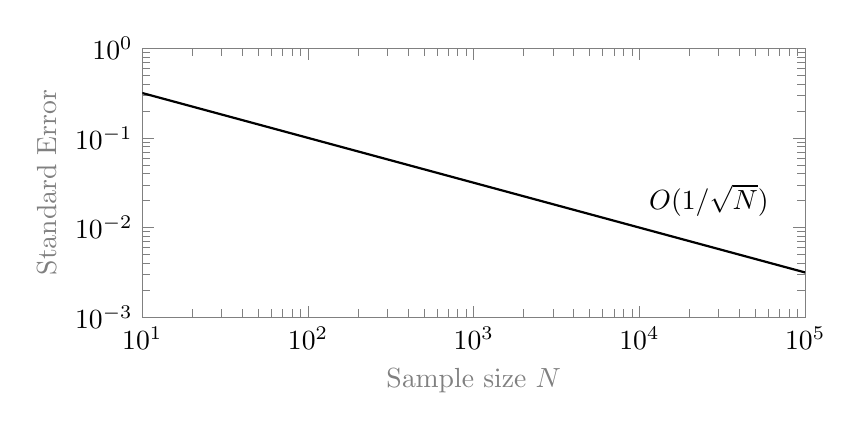
\begin{tikzpicture}
        \begin{axis}[
            width=10cm,
            height=5cm,
            xlabel={Sample size $N$},
            ylabel={Standard Error},
            xmode=log,
            ymode=log,
            xmin=10, xmax=100000,
            ymin=0.001, ymax=1,
            tick style={gray},
            label style={gray},
            axis line style={gray},
        ]
        \addplot[black, thick, domain=10:100000, samples=50] {1/sqrt(x)};
        \node[right] at (axis cs:10000, 0.02) {$O(1/\sqrt{N})$};
        \end{axis}
    \end{tikzpicture}
    \caption{Monte Carlo error decreases as $1/\sqrt{N}$, independent of dimension.}
    \label{fig:mc_error}
\end{figure}

\newthought{Comparison for $d = 100$:}
\begin{itemize}
    \item Trapezoid with $N = 10$ per dim: $10^{100}$ points---impossible
    \item Monte Carlo with $N = 10000$ points: error $\sim 0.01 \sigma_f$---easy!
\end{itemize}


\subsection{Example: Estimating $\pi$}
\index{estimating pi}

\newthought{Classic example:} Estimate $\pi$ by sampling points in $[0,1]^2$.

The area of the quarter circle is $\pi/4$. Sample $N$ uniform points and count how many fall inside:

\begin{equation}
    \hat{\pi} = 4 \cdot \frac{\#\{(x_i, y_i) : x_i^2 + y_i^2 \leq 1\}}{N}
\end{equation}

\marginnote{\newthought{The method:}
\begin{enumerate}
    \item Generate random $(x, y) \in [0,1]^2$
    \item Check if $x^2 + y^2 \leq 1$
    \item Count fraction inside
    \item Multiply by 4
\end{enumerate}}

\begin{table*}[ht]
\centering
\begin{tabular}{p{0.15\textwidth}p{0.30\textwidth}p{0.25\textwidth}}
\toprule
$N$ & Typical $|\hat{\pi} - \pi|$ & Relative Error \\
\midrule
100 & 0.15 & 5\% \\
1,000 & 0.05 & 1.6\% \\
10,000 & 0.015 & 0.5\% \\
100,000 & 0.005 & 0.16\% \\
1,000,000 & 0.0016 & 0.05\% \\
\bottomrule
\end{tabular}
\vspace{2em}
\caption{Monte Carlo estimation of $\pi$: error decreases as $1/\sqrt{N}$, requiring $100\times$ more samples for $10\times$ less error.}
\label{tab:mc_pi}
\end{table*}

The error decreases as $1/\sqrt{N}$: 100$\times$ more samples gives 10$\times$ less error.




\newpage
\section{Variance Reduction}
\index{variance reduction}

\newthought{The problem:} MC converges slowly---$O(1/\sqrt{N})$. To halve the error, we need $4\times$ more samples. Can we do better?

\newthought{Key insight:} Error $\propto \sigma_f$. Reduce the variance, reduce the error!


\subsection{Importance Sampling}
\index{importance sampling}

\newthought{Idea:} Sample more where $|f|$ is large.

Rewrite the integral:
\begin{equation}
    I = \int f(\mathbf{x}) \, d\mathbf{x} = \int \frac{f(\mathbf{x})}{q(\mathbf{x})} q(\mathbf{x}) \, d\mathbf{x} = \mathbb{E}_{\mathbf{X} \sim q}\left[\frac{f(\mathbf{X})}{q(\mathbf{X})}\right]
\end{equation}

\newthought{Importance sampling estimator:}
\begin{equation}
    \hat{I}_N = \frac{1}{N} \sum_{i=1}^{N} \frac{f(\mathbf{X}_i)}{q(\mathbf{X}_i)}, \quad \mathbf{X}_i \sim q
\end{equation}

\marginnote{\newthought{Optimal $q$:} $q^*(\mathbf{x}) \propto |f(\mathbf{x})|$ gives zero variance! But we'd need to know $\int |f|$ already, which defeats the purpose. In practice, we use an approximation to $q^*$.}

\newthought{In ML, importance sampling appears in:}
\begin{itemize}
    \item Off-policy reinforcement learning
    \item Prioritized experience replay (sample harder examples more)
    \item Hard negative mining in contrastive learning
    \item Rare event simulation
\end{itemize}


\subsection{Stratified Sampling}
\index{stratified sampling}

\newthought{Idea:} Divide domain into strata, sample from each proportionally.

\begin{enumerate}
    \item Partition $\Omega = \Omega_1 \cup \Omega_2 \cup \cdots \cup \Omega_K$
    \item Sample $N_k$ points from each $\Omega_k$
    \item Weight by stratum volume
\end{enumerate}

This ensures uniform coverage and eliminates variance from random ``clumping.''


\subsection{Control Variates}
\index{control variates}

\newthought{Idea:} Subtract a function with known mean.

If $g(\mathbf{x})$ has known expectation $\mu_g = \mathbb{E}[g(\mathbf{X})]$:
\begin{equation}
    \hat{I} = \frac{1}{N}\sum_{i=1}^N [f(\mathbf{X}_i) - c \cdot g(\mathbf{X}_i)] + c \cdot \mu_g
\end{equation}

If $g \approx f$, then $\text{Var}(f - cg) \ll \text{Var}(f)$ for appropriate $c$.

\marginnote{\newthought{Example:} To integrate $e^x$, use control variate $g(x) = 1 + x$ (linear approximation). Since $\int_0^1 (1+x)dx = 1.5$ is known, the variance of $e^x - c(1+x)$ is much smaller than $e^x$ alone.}




% ==============================================================================================
% STUDENT ACTIVATION BLOCK

\newpage
\section{Examples \& Exercises}
\index{Romberg integration!exercises}
\index{Monte Carlo!exercises}

\marginnote{\newthought{Code} can be found at \url{https://github.com/Quillstacks/lecturecode_numericalmethods.git}.}

\newthought{Exercise 1: Romberg tableau.} Build the Romberg tableau for $\int_0^{\pi} \sin(x) dx$ (true value = 2).

\textbf{Step 1:} Compute trapezoid estimates.
\begin{align*}
    T_{0,0} &= \frac{\pi}{2}[\sin(0) + \sin(\pi)] = \frac{\pi}{2}[0 + 0] = 0 \\
    T_{1,0} &= \frac{\pi/2}{2}[\sin(0) + 2\sin(\pi/2) + \sin(\pi)] = \frac{\pi}{4}[0 + 2 + 0] = \frac{\pi}{2} \approx 1.5708 \\
    T_{2,0} &= \frac{\pi/4}{2}[\sin(0) + 2\sin(\pi/4) + 2\sin(\pi/2) + 2\sin(3\pi/4) + \sin(\pi)] \\
    &= \frac{\pi}{8}[0 + 2 \cdot 0.707 + 2 + 2 \cdot 0.707 + 0] = \frac{\pi}{8} \cdot 4.828 \approx 1.8961
\end{align*}

\textbf{Step 2:} Extrapolate.
\begin{align*}
    T_{1,1} &= \frac{4 \cdot 1.5708 - 0}{3} = 2.0944 \\
    T_{2,1} &= \frac{4 \cdot 1.8961 - 1.5708}{3} = 2.0046 \\
    T_{2,2} &= \frac{16 \cdot 2.0046 - 2.0944}{15} = 1.9986
\end{align*}

After 3 rows, error is only 0.07\%!


\vspace{2em}
\newthought{Exercise 2: Monte Carlo $\pi$.} Implement the $\pi$ estimation and verify the $1/\sqrt{N}$ convergence.


\vspace{2em}
\newthought{Exercise 3: High-dimensional sphere.} The volume of a $d$-dimensional unit ball is $V_d = \pi^{d/2}/\Gamma(d/2 + 1)$.

Use Monte Carlo to estimate $V_d$ for $d = 2, 5, 10, 20$. Observe how the fraction of the hypercube occupied by the ball decreases with dimension.


\vspace{2em}
\newthought{Exercise 4: SGD as Monte Carlo.} Show that the mini-batch gradient $g_B = \frac{1}{|B|}\sum_{i \in B} \nabla \ell_i$ is an unbiased estimate of $\nabla L$. What is its variance? How does batch size affect it?




\newpage
\section{Self-Reflection and Recap}
\index{numerical integration!recap}

\newthought{Self-Reflection} Questions to guide your understanding:
\begin{itemize}
    \item Why is mini-batch SGD a Monte Carlo method?
    \item What determines the variance of your gradient estimate in SGD?
    \item Why does larger batch size give ``smoother'' training curves?
    \item When would you use Romberg vs. Monte Carlo?
    \item How does importance sampling relate to prioritized replay in RL?
    \item Why does MC error not depend on dimension?
\end{itemize}

\newthought{Recap} of Key Concepts:
\begin{itemize}
    \item \textbf{Richardson extrapolation:} Combine estimates at different $h$ to cancel error terms; jumps from $O(h^2)$ to $O(h^4)$ without new evaluations.
    \item \textbf{Romberg integration:} Apply Richardson repeatedly; build tableau of increasingly accurate estimates.
    \item \textbf{Curse of dimensionality:} Deterministic quadrature needs $O(N^d)$ points---exponential in dimension.
    \item \textbf{Monte Carlo:} Random sampling gives error $O(1/\sqrt{N})$ independent of dimension.
    \item \textbf{Variance reduction:} Importance sampling, stratification, control variates can dramatically improve MC efficiency.
    \item \textbf{SGD is MC:} Mini-batch gradients are Monte Carlo gradient estimates.
\end{itemize}


\marginnote{\newthought{Teaser.} Integration assumes we know $f(x)$ at any point we want. But \textbf{data comes as scattered samples}. We have $(x_1, y_1), \ldots, (x_n, y_n)$ and want to know $f$ between the points. How do we fill the gaps?}

\newthought{From integration to interpolation.} We've learned to compute integrals of known functions. But in data science, we often only have sample points. The next chapter explores \emph{interpolation}: reconstructing continuous functions from discrete data---the mathematical foundation of function approximation and neural networks.



%%%%%%%%%%%%%%%%%%%%%%%%%%%%%%%%%%%%%%%%%%%%%%%%%%%%%%%%%%%%%%%%%%%%%%%%%%%%%%
